\documentclass[twoside]{book}

% Packages required by doxygen
\usepackage{fixltx2e}
\usepackage{calc}
\usepackage{doxygen}
\usepackage[export]{adjustbox} % also loads graphicx
\usepackage{graphicx}
\usepackage[utf8]{inputenc}
\usepackage{makeidx}
\usepackage{multicol}
\usepackage{multirow}
\PassOptionsToPackage{warn}{textcomp}
\usepackage{textcomp}
\usepackage[nointegrals]{wasysym}
\usepackage[table]{xcolor}

% NLS support packages
\usepackage[T2A]{fontenc}
\usepackage[russian]{babel}

% Font selection
\usepackage[T1]{fontenc}
\usepackage[scaled=.90]{helvet}
\usepackage{courier}
\usepackage{amssymb}
\usepackage{sectsty}
\renewcommand{\familydefault}{\sfdefault}
\allsectionsfont{%
  \fontseries{bc}\selectfont%
  \color{darkgray}%
}
\renewcommand{\DoxyLabelFont}{%
  \fontseries{bc}\selectfont%
  \color{darkgray}%
}
\newcommand{\+}{\discretionary{\mbox{\scriptsize$\hookleftarrow$}}{}{}}

% Page & text layout
\usepackage{geometry}
\geometry{%
  a4paper,%
  top=2.5cm,%
  bottom=2.5cm,%
  left=2.5cm,%
  right=2.5cm%
}
\tolerance=750
\hfuzz=15pt
\hbadness=750
\setlength{\emergencystretch}{15pt}
\setlength{\parindent}{0cm}
\setlength{\parskip}{3ex plus 2ex minus 2ex}
\makeatletter
\renewcommand{\paragraph}{%
  \@startsection{paragraph}{4}{0ex}{-1.0ex}{1.0ex}{%
    \normalfont\normalsize\bfseries\SS@parafont%
  }%
}
\renewcommand{\subparagraph}{%
  \@startsection{subparagraph}{5}{0ex}{-1.0ex}{1.0ex}{%
    \normalfont\normalsize\bfseries\SS@subparafont%
  }%
}
\makeatother

% Headers & footers
\usepackage{fancyhdr}
\pagestyle{fancyplain}
\fancyhead[LE]{\fancyplain{}{\bfseries\thepage}}
\fancyhead[CE]{\fancyplain{}{}}
\fancyhead[RE]{\fancyplain{}{\bfseries\leftmark}}
\fancyhead[LO]{\fancyplain{}{\bfseries\rightmark}}
\fancyhead[CO]{\fancyplain{}{}}
\fancyhead[RO]{\fancyplain{}{\bfseries\thepage}}
\fancyfoot[LE]{\fancyplain{}{}}
\fancyfoot[CE]{\fancyplain{}{}}
\fancyfoot[RE]{\fancyplain{}{\bfseries\scriptsize Создано системой Doxygen }}
\fancyfoot[LO]{\fancyplain{}{\bfseries\scriptsize Создано системой Doxygen }}
\fancyfoot[CO]{\fancyplain{}{}}
\fancyfoot[RO]{\fancyplain{}{}}
\renewcommand{\footrulewidth}{0.4pt}
\renewcommand{\chaptermark}[1]{%
  \markboth{#1}{}%
}
\renewcommand{\sectionmark}[1]{%
  \markright{\thesection\ #1}%
}

% Indices & bibliography
\usepackage{natbib}
\usepackage[titles]{tocloft}
\setcounter{tocdepth}{3}
\setcounter{secnumdepth}{5}
\makeindex

% Hyperlinks (required, but should be loaded last)
\usepackage{ifpdf}
\ifpdf
  \usepackage[pdftex,pagebackref=true]{hyperref}
\else
  \usepackage[ps2pdf,pagebackref=true]{hyperref}
\fi
\hypersetup{%
  colorlinks=true,%
  linkcolor=blue,%
  citecolor=blue,%
  unicode%
}

% Custom commands
\newcommand{\clearemptydoublepage}{%
  \newpage{\pagestyle{empty}\cleardoublepage}%
}

\usepackage{caption}
\captionsetup{labelsep=space,justification=centering,font={bf},singlelinecheck=off,skip=4pt,position=top}

%===== C O N T E N T S =====

\begin{document}

% Titlepage & ToC
\hypersetup{pageanchor=false,
             bookmarksnumbered=true,
             pdfencoding=unicode
            }
\pagenumbering{alph}
\begin{titlepage}
\vspace*{7cm}
\begin{center}%
{\Large Шифр маршрутной перестановки }\\
\vspace*{1cm}
{\large Создано системой Doxygen 1.8.13}\\
\end{center}
\end{titlepage}
\clearemptydoublepage
\pagenumbering{roman}
\tableofcontents
\clearemptydoublepage
\pagenumbering{arabic}
\hypersetup{pageanchor=true}

%--- Begin generated contents ---
\chapter{Иерархический список классов}
\section{Иерархия классов}
Иерархия классов.\begin{DoxyCompactList}
\item invalid\+\_\+argument\begin{DoxyCompactList}
\item \contentsline{section}{cipher\+\_\+error}{\pageref{classcipher__error}}{}
\end{DoxyCompactList}
\item \contentsline{section}{mod\+Alpha\+Cipher}{\pageref{classmodAlphaCipher}}{}
\end{DoxyCompactList}

\chapter{Алфавитный указатель классов}
\section{Классы}
Классы с их кратким описанием.\begin{DoxyCompactList}
\item\contentsline{section}{\hyperlink{classcipher__error}{cipher\+\_\+error} }{\pageref{classcipher__error}}{}
\item\contentsline{section}{\hyperlink{classmodAlphaCipher}{mod\+Alpha\+Cipher} \\*Шифрование методом Гронсфельда }{\pageref{classmodAlphaCipher}}{}
\end{DoxyCompactList}

\chapter{Список файлов}
\section{Файлы}
Полный список документированных файлов.\begin{DoxyCompactList}
\item\contentsline{section}{\hyperlink{main_8cpp}{main.\+cpp} \\*Главный файл для модуля swapcipher }{\pageref{main_8cpp}}{}
\item\contentsline{section}{\hyperlink{swapcipher_8cpp}{swapcipher.\+cpp} \\*Исполняемый файл для модуля swapcipher }{\pageref{swapcipher_8cpp}}{}
\item\contentsline{section}{\hyperlink{swapcipher_8h}{swapcipher.\+h} \\*Заголовочный файл для модуля swapcipher }{\pageref{swapcipher_8h}}{}
\end{DoxyCompactList}

\chapter{Классы}
\hypertarget{classcipher__error}{}\section{Класс cipher\+\_\+error}
\label{classcipher__error}\index{cipher\+\_\+error@{cipher\+\_\+error}}


Граф наследования\+:cipher\+\_\+error\+:\nopagebreak
\begin{figure}[H]
\begin{center}
\leavevmode
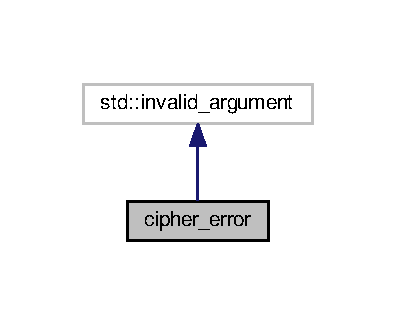
\includegraphics[width=190pt]{classcipher__error__inherit__graph}
\end{center}
\end{figure}


Граф связей класса cipher\+\_\+error\+:\nopagebreak
\begin{figure}[H]
\begin{center}
\leavevmode
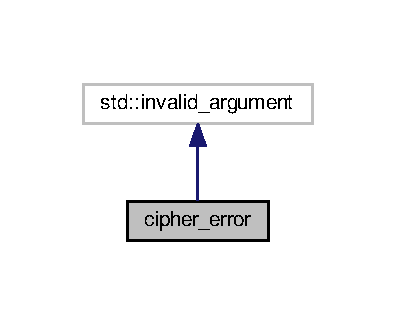
\includegraphics[width=190pt]{classcipher__error__coll__graph}
\end{center}
\end{figure}
\subsection*{Открытые члены}
\begin{DoxyCompactItemize}
\item 
\mbox{\Hypertarget{classcipher__error_aac662e216a84bfeb873303c7b88d029e}\label{classcipher__error_aac662e216a84bfeb873303c7b88d029e}} 
{\bfseries cipher\+\_\+error} (const std\+::string \&what\+\_\+arg)
\item 
\mbox{\Hypertarget{classcipher__error_a18cf27d9c2cd2538d3cb8f17e9a55f3e}\label{classcipher__error_a18cf27d9c2cd2538d3cb8f17e9a55f3e}} 
{\bfseries cipher\+\_\+error} (const char $\ast$what\+\_\+arg)
\end{DoxyCompactItemize}


Объявления и описания членов класса находятся в файле\+:\begin{DoxyCompactItemize}
\item 
\hyperlink{modAlphaCipher_8h}{mod\+Alpha\+Cipher.\+h}\end{DoxyCompactItemize}

\hypertarget{classSwapCipher}{}\section{Класс Swap\+Cipher}
\label{classSwapCipher}\index{Swap\+Cipher@{Swap\+Cipher}}


Шифрование методом табличной перестановки  




{\ttfamily \#include $<$swapcipher.\+h$>$}

\subsection*{Открытые члены}
\begin{DoxyCompactItemize}
\item 
\mbox{\Hypertarget{classSwapCipher_a833505a4c3a4e35bd29221fdc0721479}\label{classSwapCipher_a833505a4c3a4e35bd29221fdc0721479}} 
\hyperlink{classSwapCipher_a833505a4c3a4e35bd29221fdc0721479}{Swap\+Cipher} ()=delete
\begin{DoxyCompactList}\small\item\em конструктор без параметров запрещен \end{DoxyCompactList}\item 
\mbox{\Hypertarget{classSwapCipher_ad13cc690789eb715e51b2dc6b002c494}\label{classSwapCipher_ad13cc690789eb715e51b2dc6b002c494}} 
\hyperlink{classSwapCipher_ad13cc690789eb715e51b2dc6b002c494}{Swap\+Cipher} (const int key1)
\begin{DoxyCompactList}\small\item\em конструктор для установки ключа \end{DoxyCompactList}\item 
std\+::string \hyperlink{classSwapCipher_adab0495fb3203c0214143969d9945573}{encrypt} (const std\+::string \&open\+\_\+text)
\begin{DoxyCompactList}\small\item\em Зашифровывание \end{DoxyCompactList}\item 
std\+::string \hyperlink{classSwapCipher_a198011fc3328030ef7c2493cd0b5abeb}{decrypt} (const std\+::string \&cipher\+\_\+text)
\begin{DoxyCompactList}\small\item\em Дешифровывание \end{DoxyCompactList}\end{DoxyCompactItemize}
\subsection*{Закрытые члены}
\begin{DoxyCompactItemize}
\item 
void \hyperlink{classSwapCipher_a7b86880b1a197343bcf65a395c2d3d2e}{get\+Valid\+Key} (const int \&key)
\begin{DoxyCompactList}\small\item\em Проверка ключа на валидность \end{DoxyCompactList}\item 
std\+::string \hyperlink{classSwapCipher_aeee71718a56980b964abc32cda498a98}{get\+Valid\+Open\+Text} (const std\+::string \&s)
\begin{DoxyCompactList}\small\item\em Проверка шифруемого текста \end{DoxyCompactList}\item 
std\+::string \hyperlink{classSwapCipher_a243f5c096f4cd4b0f4d4b7993fb082d6}{get\+Valid\+Cipher\+Text} (const std\+::string \&s)
\begin{DoxyCompactList}\small\item\em Проверка дешифруемого текста \end{DoxyCompactList}\end{DoxyCompactItemize}
\subsection*{Закрытые данные}
\begin{DoxyCompactItemize}
\item 
\mbox{\Hypertarget{classSwapCipher_a2f19bca4df89af5479700ed57a976bb2}\label{classSwapCipher_a2f19bca4df89af5479700ed57a976bb2}} 
int \hyperlink{classSwapCipher_a2f19bca4df89af5479700ed57a976bb2}{key\+\_\+stolbec}
\begin{DoxyCompactList}\small\item\em ключ(количество столбцов матрицы) \end{DoxyCompactList}\item 
\mbox{\Hypertarget{classSwapCipher_afdbad1d138089f2e2e6bcf40dc53e18f}\label{classSwapCipher_afdbad1d138089f2e2e6bcf40dc53e18f}} 
int \hyperlink{classSwapCipher_afdbad1d138089f2e2e6bcf40dc53e18f}{key\+\_\+stroka}
\begin{DoxyCompactList}\small\item\em количество строк матрицы \end{DoxyCompactList}\item 
\mbox{\Hypertarget{classSwapCipher_a784b1cc877aac8c85a4586c2e46f5906}\label{classSwapCipher_a784b1cc877aac8c85a4586c2e46f5906}} 
std\+::wstring \hyperlink{classSwapCipher_a784b1cc877aac8c85a4586c2e46f5906}{real\+\_\+cp}
\begin{DoxyCompactList}\small\item\em строка передающаяся в decrypt. \end{DoxyCompactList}\end{DoxyCompactItemize}


\subsection{Подробное описание}
Шифрование методом табличной перестановки 

Ключ устанавливается в конструкторе. Для зашифровывания и расшифровывания предназначены методы encrypt и decrypt. \begin{DoxyWarning}{Предупреждения}
Реализация только для русского языка 
\end{DoxyWarning}


\subsection{Методы}
\mbox{\Hypertarget{classSwapCipher_a198011fc3328030ef7c2493cd0b5abeb}\label{classSwapCipher_a198011fc3328030ef7c2493cd0b5abeb}} 
\index{Swap\+Cipher@{Swap\+Cipher}!decrypt@{decrypt}}
\index{decrypt@{decrypt}!Swap\+Cipher@{Swap\+Cipher}}
\subsubsection{\texorpdfstring{decrypt()}{decrypt()}}
{\footnotesize\ttfamily std\+::string Swap\+Cipher\+::decrypt (\begin{DoxyParamCaption}\item[{const std\+::string \&}]{cipher\+\_\+text }\end{DoxyParamCaption})}



Дешифровывание 


\begin{DoxyParams}[1]{Аргументы}
\mbox{\tt in}  & {\em open\+\_\+text} & Закодированный текст. Не должен быть пустой строкой. Не должен быть единичной длины \\
\hline
\end{DoxyParams}
\begin{DoxyReturn}{Возвращает}
Зашифрованная строка 
\end{DoxyReturn}

\begin{DoxyExceptions}{Исключения}
{\em \hyperlink{classcipher__error}{cipher\+\_\+error},если} & текст пустой если текст еденичной длины если текст содержит пробелы \\
\hline
\end{DoxyExceptions}
\mbox{\Hypertarget{classSwapCipher_adab0495fb3203c0214143969d9945573}\label{classSwapCipher_adab0495fb3203c0214143969d9945573}} 
\index{Swap\+Cipher@{Swap\+Cipher}!encrypt@{encrypt}}
\index{encrypt@{encrypt}!Swap\+Cipher@{Swap\+Cipher}}
\subsubsection{\texorpdfstring{encrypt()}{encrypt()}}
{\footnotesize\ttfamily std\+::string Swap\+Cipher\+::encrypt (\begin{DoxyParamCaption}\item[{const std\+::string \&}]{open\+\_\+text }\end{DoxyParamCaption})}



Зашифровывание 


\begin{DoxyParams}[1]{Аргументы}
\mbox{\tt in}  & {\em open\+\_\+text} & Открытый текст. Не должен быть пустой строкой. Не должен быть единичной длины Строчные символы автоматически преобразуются к прописным. \\
\hline
\end{DoxyParams}
\begin{DoxyReturn}{Возвращает}
Зашифрованная строка 
\end{DoxyReturn}

\begin{DoxyExceptions}{Исключения}
{\em \hyperlink{classcipher__error}{cipher\+\_\+error},если} & текст пустой если текст еденичной длины если текст содержит пробелы \\
\hline
\end{DoxyExceptions}
\mbox{\Hypertarget{classSwapCipher_a243f5c096f4cd4b0f4d4b7993fb082d6}\label{classSwapCipher_a243f5c096f4cd4b0f4d4b7993fb082d6}} 
\index{Swap\+Cipher@{Swap\+Cipher}!get\+Valid\+Cipher\+Text@{get\+Valid\+Cipher\+Text}}
\index{get\+Valid\+Cipher\+Text@{get\+Valid\+Cipher\+Text}!Swap\+Cipher@{Swap\+Cipher}}
\subsubsection{\texorpdfstring{get\+Valid\+Cipher\+Text()}{getValidCipherText()}}
{\footnotesize\ttfamily std\+::string Swap\+Cipher\+::get\+Valid\+Cipher\+Text (\begin{DoxyParamCaption}\item[{const std\+::string \&}]{s }\end{DoxyParamCaption})\hspace{0.3cm}{\ttfamily [inline]}, {\ttfamily [private]}}



Проверка дешифруемого текста 

Проверки на все исключения \char`\"{}выбрасываеые\char`\"{} методом decrypt 
\begin{DoxyParams}[1]{Аргументы}
\mbox{\tt in}  & {\em cipher\+\_\+text} & Зашифрованный текст. \\
\hline
\end{DoxyParams}

\begin{DoxyExceptions}{Исключения}
{\em \hyperlink{classcipher__error}{cipher\+\_\+error},если} & текст пустой если текст еденичной длины если текст содержит пробелы \\
\hline
\end{DoxyExceptions}
\mbox{\Hypertarget{classSwapCipher_a7b86880b1a197343bcf65a395c2d3d2e}\label{classSwapCipher_a7b86880b1a197343bcf65a395c2d3d2e}} 
\index{Swap\+Cipher@{Swap\+Cipher}!get\+Valid\+Key@{get\+Valid\+Key}}
\index{get\+Valid\+Key@{get\+Valid\+Key}!Swap\+Cipher@{Swap\+Cipher}}
\subsubsection{\texorpdfstring{get\+Valid\+Key()}{getValidKey()}}
{\footnotesize\ttfamily void Swap\+Cipher\+::get\+Valid\+Key (\begin{DoxyParamCaption}\item[{const int \&}]{key }\end{DoxyParamCaption})\hspace{0.3cm}{\ttfamily [private]}}



Проверка ключа на валидность 

Проверки на все исключения \char`\"{}выбрасываеые\char`\"{} конструктором 
\begin{DoxyParams}[1]{Аргументы}
\mbox{\tt in}  & {\em key} & Ключ. \\
\hline
\end{DoxyParams}

\begin{DoxyExceptions}{Исключения}
{\em \hyperlink{classcipher__error}{cipher\+\_\+error}} & если ключ -\/ меньше нуля или ноль. \\
\hline
\end{DoxyExceptions}
\mbox{\Hypertarget{classSwapCipher_aeee71718a56980b964abc32cda498a98}\label{classSwapCipher_aeee71718a56980b964abc32cda498a98}} 
\index{Swap\+Cipher@{Swap\+Cipher}!get\+Valid\+Open\+Text@{get\+Valid\+Open\+Text}}
\index{get\+Valid\+Open\+Text@{get\+Valid\+Open\+Text}!Swap\+Cipher@{Swap\+Cipher}}
\subsubsection{\texorpdfstring{get\+Valid\+Open\+Text()}{getValidOpenText()}}
{\footnotesize\ttfamily std\+::string Swap\+Cipher\+::get\+Valid\+Open\+Text (\begin{DoxyParamCaption}\item[{const std\+::string \&}]{s }\end{DoxyParamCaption})\hspace{0.3cm}{\ttfamily [inline]}, {\ttfamily [private]}}



Проверка шифруемого текста 

Проверки на все исключения \char`\"{}выбрасываеые\char`\"{} методом encrypt 
\begin{DoxyParams}[1]{Аргументы}
\mbox{\tt in}  & {\em open\+\_\+text} & Открытый текст. \\
\hline
\end{DoxyParams}

\begin{DoxyExceptions}{Исключения}
{\em \hyperlink{classcipher__error}{cipher\+\_\+error},если} & текст пустой если текст еденичной длины если текст содержит пробелы \\
\hline
\end{DoxyExceptions}


Объявления и описания членов классов находятся в файлах\+:\begin{DoxyCompactItemize}
\item 
\hyperlink{swapcipher_8h}{swapcipher.\+h}\item 
\hyperlink{swapcipher_8cpp}{swapcipher.\+cpp}\end{DoxyCompactItemize}

\chapter{Файлы}
\hypertarget{main_8cpp}{}\section{Файл main.\+cpp}
\label{main_8cpp}\index{main.\+cpp@{main.\+cpp}}


Главный файл для модуля swapcipher.  


{\ttfamily \#include $<$iostream$>$}\newline
{\ttfamily \#include \char`\"{}swapcipher.\+h\char`\"{}}\newline
Граф включаемых заголовочных файлов для main.\+cpp\+:\nopagebreak
\begin{figure}[H]
\begin{center}
\leavevmode
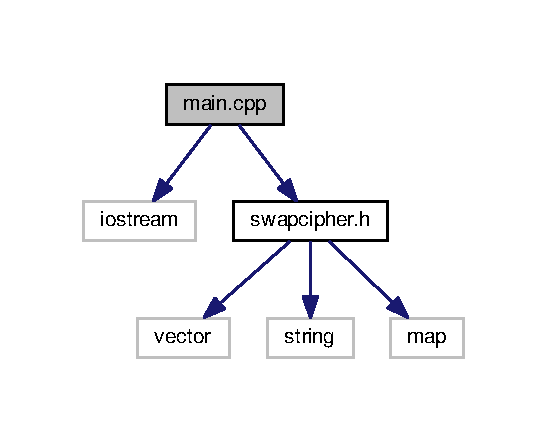
\includegraphics[width=263pt]{main_8cpp__incl}
\end{center}
\end{figure}
\subsection*{Функции}
\begin{DoxyCompactItemize}
\item 
\mbox{\Hypertarget{main_8cpp_a66bfb6c3fdd823120a3614d831375e22}\label{main_8cpp_a66bfb6c3fdd823120a3614d831375e22}} 
void {\bfseries check} (const string \&Text, const int key, const bool destruct\+Cipher\+Text=false)
\item 
\mbox{\Hypertarget{main_8cpp_a3c04138a5bfe5d72780bb7e82a18e627}\label{main_8cpp_a3c04138a5bfe5d72780bb7e82a18e627}} 
int {\bfseries main} (int argc, char $\ast$$\ast$argv)
\end{DoxyCompactItemize}


\subsection{Подробное описание}
Главный файл для модуля swapcipher. 

\begin{DoxyAuthor}{Автор}
Григорьев А.\+Д. 
\end{DoxyAuthor}
\begin{DoxyVersion}{Версия}
1.\+0 
\end{DoxyVersion}
\begin{DoxyDate}{Дата}
09.\+06.\+2019 
\end{DoxyDate}
\begin{DoxyCopyright}{Авторство}
ИБСТ ПГУ 
\end{DoxyCopyright}
\begin{DoxyWarning}{Предупреждения}
Это учебный пример 
\end{DoxyWarning}

\hypertarget{swapcipher_8cpp}{}\section{Файл swapcipher.\+cpp}
\label{swapcipher_8cpp}\index{swapcipher.\+cpp@{swapcipher.\+cpp}}


Исполняемый файл для модуля swapcipher.  


{\ttfamily \#include \char`\"{}swapcipher.\+h\char`\"{}}\newline
{\ttfamily \#include $<$locale$>$}\newline
{\ttfamily \#include $<$codecvt$>$}\newline
Граф включаемых заголовочных файлов для swapcipher.\+cpp\+:\nopagebreak
\begin{figure}[H]
\begin{center}
\leavevmode
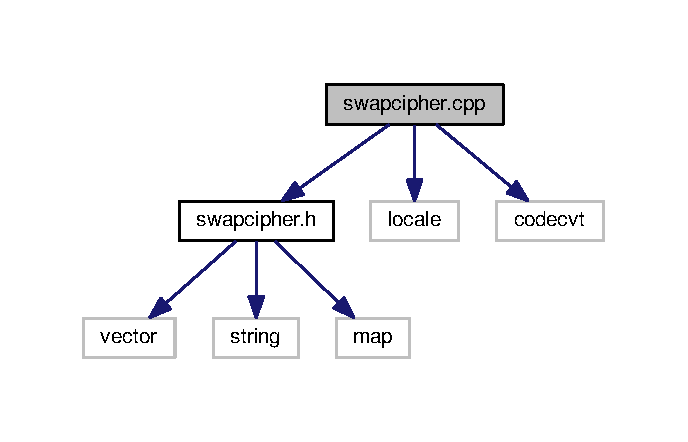
\includegraphics[width=330pt]{swapcipher_8cpp__incl}
\end{center}
\end{figure}
\subsection*{Функции}
\begin{DoxyCompactItemize}
\item 
\mbox{\Hypertarget{swapcipher_8cpp_a17741b6032756170697a03716e313030}\label{swapcipher_8cpp_a17741b6032756170697a03716e313030}} 
std\+::locale {\bfseries loc} (\char`\"{}ru\+\_\+\+R\+U.\+U\+TF-\/8\char`\"{})
\end{DoxyCompactItemize}
\subsection*{Переменные}
\begin{DoxyCompactItemize}
\item 
\mbox{\Hypertarget{swapcipher_8cpp_a6a1286b5d70cf45335abb5c1f604db4a}\label{swapcipher_8cpp_a6a1286b5d70cf45335abb5c1f604db4a}} 
std\+::wstring\+\_\+convert$<$ std\+::codecvt\+\_\+utf8$<$ wchar\+\_\+t $>$, wchar\+\_\+t $>$ {\bfseries codec}
\end{DoxyCompactItemize}


\subsection{Подробное описание}
Исполняемый файл для модуля swapcipher. 

\begin{DoxyAuthor}{Автор}
Григорьев А.\+Д. 
\end{DoxyAuthor}
\begin{DoxyVersion}{Версия}
1.\+0 
\end{DoxyVersion}
\begin{DoxyDate}{Дата}
09.\+06.\+2019 
\end{DoxyDate}
\begin{DoxyCopyright}{Авторство}
ИБСТ ПГУ 
\end{DoxyCopyright}
\begin{DoxyWarning}{Предупреждения}
Это учебный пример 
\end{DoxyWarning}

\hypertarget{swapcipher_8h}{}\section{Файл swapcipher.\+h}
\label{swapcipher_8h}\index{swapcipher.\+h@{swapcipher.\+h}}


Заголовочный файл для модуля swapcipher.  


{\ttfamily \#include $<$vector$>$}\newline
{\ttfamily \#include $<$string$>$}\newline
{\ttfamily \#include $<$map$>$}\newline
Граф включаемых заголовочных файлов для swapcipher.\+h\+:\nopagebreak
\begin{figure}[H]
\begin{center}
\leavevmode
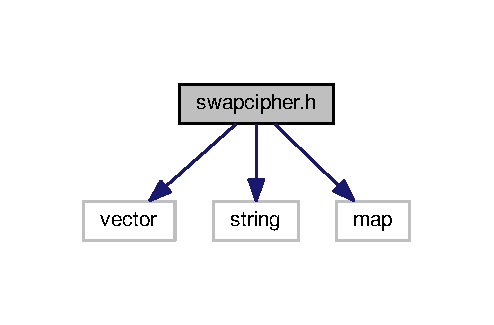
\includegraphics[width=237pt]{swapcipher_8h__incl}
\end{center}
\end{figure}
Граф файлов, в которые включается этот файл\+:
\nopagebreak
\begin{figure}[H]
\begin{center}
\leavevmode
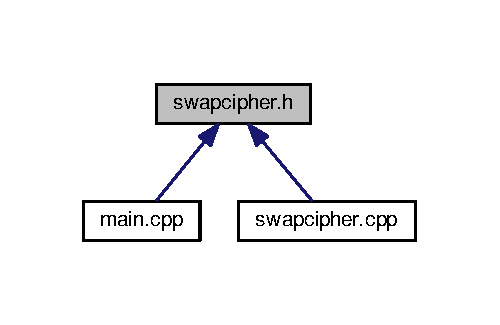
\includegraphics[width=240pt]{swapcipher_8h__dep__incl}
\end{center}
\end{figure}
\subsection*{Классы}
\begin{DoxyCompactItemize}
\item 
class \hyperlink{classSwapCipher}{Swap\+Cipher}
\begin{DoxyCompactList}\small\item\em Шифрование методом табличной перестановки \end{DoxyCompactList}\item 
class \hyperlink{classcipher__error}{cipher\+\_\+error}
\begin{DoxyCompactList}\small\item\em Класс для обработки исключений \end{DoxyCompactList}\end{DoxyCompactItemize}


\subsection{Подробное описание}
Заголовочный файл для модуля swapcipher. 

\begin{DoxyAuthor}{Автор}
Григорьев А.\+Д. 
\end{DoxyAuthor}
\begin{DoxyVersion}{Версия}
1.\+0 
\end{DoxyVersion}
\begin{DoxyDate}{Дата}
09.\+06.\+2019 
\end{DoxyDate}
\begin{DoxyCopyright}{Авторство}
ИБСТ ПГУ 
\end{DoxyCopyright}
\begin{DoxyWarning}{Предупреждения}
Это учебный пример 
\end{DoxyWarning}

%--- End generated contents ---

% Index
\backmatter
\newpage
\phantomsection
\clearemptydoublepage
\addcontentsline{toc}{chapter}{Алфавитный указатель}
\printindex

\end{document}
